\documentclass[../main.tex]{subfiles}
\begin{document}
\setchapterstyle{kao}
\setchapterpreamble[u]{\margintoc}
\setchapterimage[6.5cm]{Images/propagators.png}
\chapter[Propagators]{Propagators\footnotemark[0]}
\labch{Propagators}
\section{Green's function}
We look at the Klein-Gordon equation [\refeq{KG}] in the presence of a current:
\[
(\partial^2+m^2)\Phi(x)=J(x)
\]
and we want to find a solution in the form:
\begin{equation}
\labeq{Greenfunc}
(\partial^2+m^2)G(x,x')=\delta^4(x-x')
\end{equation}
In this way we obtain $\Phi=\Phi_0+\int d^4x'G(x,x')J(x')$, where $\Phi_0$ is the solution of the homogeneous equation. It is easy to check that this is the correct solution:
\begin{align*}
J(x)&=(\partial^2+m^2)\left(\Phi_0+\int d^4x'G(x,x')J(x')\right)\\
&=\cancelto{0}{(\partial^2+m^2)\Phi_0}+\int d^4x'(\partial^2+m^2)G(x,x')J(x')\\
&=\int d^4x'\delta^4(x-x')J(x')=J(x) \quad \checkmark
\end{align*}
The problem now becomes finding such function $G(x,x')$. The strategy is to perform a \href{https://en.wikipedia.org/wiki/Fourier_transform}{Fourier transform}, move to a solvable algebraic equation and then anti-transform:
\[
G(x,x')=\frac{1}{(2\pi)^4}\int d^4pe^{-iP_\mu(x-x')^\mu}\Tilde{G}(\underline{p}) \quad \delta^4(x-x')=\frac{1}{(2\pi)^4}\int d^4pe^{-iP_\mu(x-x')^\mu}
\]
In this way, \refeq{Greenfunc} can be written as:
\[
(-P^2+m^2)\Tilde{G}(\underline{p})=1
\]
$\Tilde{G}(\underline{p})$ is the \textbf{Green's function} and it is possible to compute it by integrating in the complex plane:
\[
G(x,x')=\frac{1}{(2\pi)^4}\int d^4pe^{-iP_\mu(x-x')^\mu}\Tilde{G}(\underline{p})=-\frac{1}{(2\pi)^4}\int d^4p\frac{e^{-iP_\mu(x-x')^\mu}}{P^2-m^2}
\]
It has poles in $P^0=\pm\sqrt{p^2+m^2}=\pm\omega_p$.
We integrate over the two circumferences $C^+$ and $C^-$ around the two poles:
\begin{figure}[h!]
    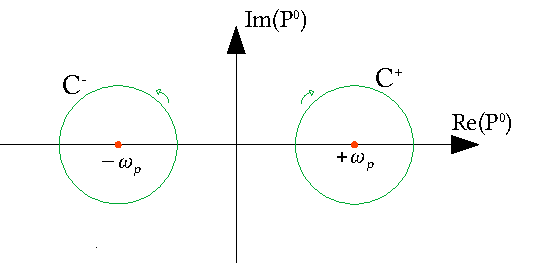
\includegraphics{Images/CamminiIntegrazione.pdf}
    \caption*{To compute the integrals, we use the \href{https://en.wikipedia.org/wiki/Residue_theorem}{Residue theorem}:\\ $\oint_\gamma dzf(z)=2\pi i\sum\text{Res}(f,a_k)$ with the residue Res$(f,c)$ defined as:\\$\frac{1}{(n-1)!}\lim_{z\to c}\frac{d^{n-1}}{dz^{n-1}}[f(z)(z-c)^n]$}
    \labfig{integrazione}
\end{figure}\\
\noindent
Integrating over $C^+$ gives us $\Delta^+(x)$
\begin{align*}
\Delta^+(x)&:=-i\int_{C^+}\frac{d^4p}{(2\pi)^4}\frac{e^{-iP_\mu x^\mu}}{P^2-m^2}=-i\int\frac{d^3p}{(2\pi)^3}\int_{C^+}\frac{dP^0}{2\pi}\frac{e^{-iP_\mu x^\mu}}{(P^0-\omega_p)(P^0+\omega_p)}\\
&=\int\frac{d^3p}{(2\pi)^3}\frac{e^{-i(\omega_pt-\underline{p}\cdot\underline{x})}}{2\omega_p}
\end{align*}
Analogously, by integrating over $C^-$ we obtain:
\[
\Delta^-(x):=-\int\frac{d^3p}{(2\pi)^3}\frac{e^{+i(\omega_pt+\underline{p}\cdot\underline{x})}}{2\omega_p}
\]
It is possible to show that $\Delta^\pm(x)$ are solutions of the homogeneous equation:
\begin{align*}
(\partial^2+m^2)\Delta^\pm(x)&=-i\int\frac{d^4p}{(2\pi)^4}\frac{(\partial^2+m^2)e^{-iP_\mu x^\mu}}{P^2-m^2}\\
&=-i\int\frac{d^3p}{(2\pi)^3}\int_{C^\pm}\frac{dP^0}{2\pi}\cancelto{-1}{\frac{(-P^2+m^2)}{P^2-m^2}}e^{-iP_\mu x^\mu}=0\quad \checkmark\marginnote{We are integrating an analytical function over closed paths containing no poles.}
\end{align*}
\subsection{Retarded and advanced Green's function}
These paths give a solution to the inhomogeneous equation. Two different paths give the same result if it is possible to continuously deform one path into another without encountering any singular point of $\Tilde{G}(p)$.
\[
\Tilde{G}(p)=\frac{e^{-iP_\mu(x-x')^\mu}}{(P^0+i\eta)^2-p^2-m^2}=\frac{e^{-iP_\mu(x-x')^\mu}}{(P^0-\omega_p+i\eta)(P^0+\omega_p+i\eta)}
\]
The \textbf{retarded Green's function} $G_{ret}$ corresponds to the condition that $G(x)=0$ for $t-t'<0$, i.e. we integrate over the upper path where we have no singularities: $G_{ret}(x-x')=0$. If instead $t-t'>0$, we integrate over the lower path:
\begin{figure}[h!]
    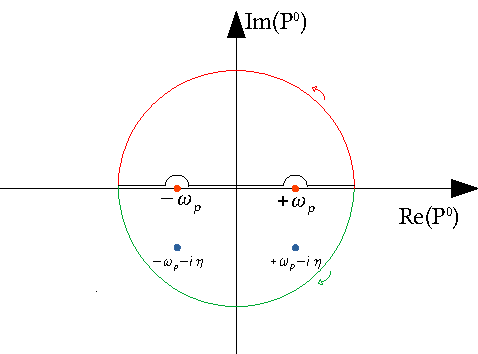
\includegraphics{Images/Greenfunction.pdf}
    \caption*{}
    \labfig{Greenfunction}    
\end{figure}
\begin{align*}
G_{ret}(x-x')&=-\frac{\theta(x^0-x'^0)}{(2\pi)^4}\int d^4p\frac{e^{-iP_\mu(x-x')^\mu}}{(P^0+i\eta)^2-p^2-m^2}\\
&=-\frac{\theta(x^0-x'^0)}{(2\pi)^4}\int d^3pe^{-i\underline{p}\cdot(\underline{x}-\underline{x}')}\int dP^0\frac{e^{-iP^0(x^0-x'^0)}}{(P^0-\omega_p+i\eta)(P^0+\omega_p+i\eta)}\\
&=-\frac{\theta(x^0-x'^0)}{(2\pi)^4}\int d^3pe^{-i\underline{p}\cdot(\underline{x}-\underline{x}')}\int \frac{dP^0}{2\omega_p}e^{-iP^0(x^0-x'^0)}\left(\frac{1}{P^0-\omega_p+i\eta}-\frac{1}{P^0+\omega_p+i\eta}\right)\\
&=\frac{i\theta(x^0-x'^0)}{(2\pi)^3}\int\frac{d^3p}{2\omega_p}\left[{\color{red}e^{-i\omega_p(x^0-x'^0)+i\underline{p}\cdot(\underline{x}-\underline{x}')}}-{\color{blue}e^{+i\omega_p(x^0-x'^0)+i\underline{p}\cdot(\underline{x}-\underline{x}')}}\right]\\
&=\theta(x^0-x'^0)[i{\color{red}\Delta^+(x-x')}+i{\color{blue}\Delta^-(x-x')}]
\end{align*}
This means that the positive and negative energy solutions are both transposed \textbf{forward} in time.

If we consider the case with the two roots displaced in the upper plane, we get that $G(x)=0$ for $t-t'>0$ because we are integrating in the lower plane which contains no singularities. For $t-t'<0$ we are instead in the upper plane, skipping the calculations (which are the same as before) we obtain that the \textbf{advanced Green's function} is defined as:
\[
G_{adv}(x-x')=-\theta(x^0-x'^0)[i\Delta^+(x-x')+i\Delta^-(x-x')]
\]
This means that positive and negative energy solutions are both transposed \textbf{backwards} in time. The goal now is to find the same solution for a quantum field. It is trivial to understand that moving the positive energy solution forward in time is consistent with causality, because we know that the particle is the positive energy solution: the negative energy solution is linked to the anti-particle.
\section{Feynman propagator}
In order to select the path that gives us positive energy solutions and propagation forward in time, we use the \textbf{Feynman propagator}. This is obtained from the condition coinciding with $i\Delta^+(x)$ for $t-t'>0$ and $i\Delta^-(x)$ for $t-t'<0$. This condition originates the following integration path:
\begin{figure}[h!]
    \centering
    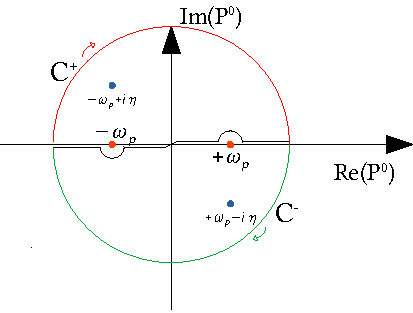
\includegraphics{Images/CamminiIntegrazioneFeynman.pdf}
    \caption*{}
    \labfig{Feynamnpropagator}
\end{figure}
\begin{align*}
D_F(x-x')&=-\int\frac{d^4p}{(2\pi)^4}\frac{e^{-iP_\mu(x-x')^\mu}}{P^2-m^2}\\
&=-\frac{\theta(x^0-x'^0)}{(2\pi)^4}\int\frac{d^3p}{2\omega_p}e^{i\underline{p}\cdot(\underline{x}-\underline{x}')}\int_{{\color{green}C^-}} dP^0e^{-iP^0(x^0-x'^0)}\left[\frac{1}{P^0-\omega_p+i\eta}-\frac{1}{P^0+\omega_p+i\eta}\right]\\
&-\frac{\theta(x'^0-x^0)}{(2\pi)^4}\int\frac{d^3p}{2\omega_p}e^{i\underline{p}\cdot(\underline{x}-\underline{x}')}\int_{{\color{red}C^+}} dP^0e^{-iP^0(x^0-x'^0)}\left[\frac{1}{P^0-\omega_p+i\eta}-\frac{1}{P^0+\omega_p+i\eta}\right]\\
&=i\theta(x^0-x'^0)\int\frac{d^3p}{(2\pi)^3}\frac{e^{-iP_\mu(x-x')^\mu}}{2\omega_p}+i\theta(x'^0-x^0)\int\frac{d^3p}{(2\pi)^3}\frac{e^{iP_\mu(x-x')^\mu}}{2\omega_p}\\
&=D_f(x-x')=\theta(x^0-x'^0)i\Delta^+(x-x')-\theta(x'^0-x^0)i\Delta^-(x-x')
\end{align*}
Consider the following process: a boson is created in a certain point $(\underline{x},t)$, we want to know what is the probability amplitude to have this particle in a point $(\underline{y},t')$ with $t'>t$. Keeping in mind that 
\[
\Phi(x)=\int d^3p[a(p)f^+(p)+b^\dagger(p)f^{+*}(p)]
\]
we want to create a charge +1 in $(\underline{x},t)$:
\begin{align*}
\ket{\Psi(\underline{x},t)}&=\Phi^\dagger(x)\ket{0}=\int d^3p[f_p^\dagger \cancelto{0}{b(p)\ket{0}}+f_p^{(+)\dagger}a^\dagger(p)\ket{0}]\\
&=\int \frac{d^3p}{(2\pi)^{3/2}}\frac{e^{iP_\mu x^\mu}}{\sqrt{2\omega_p}}a^\dagger(p)\ket{0}
\end{align*}
If, as we stated, the point $(\underline{y},t')$ is such that $t'>t$, the probability amplitude is:
\[
\theta(t'-t)\bra{\Psi(\underline{y},t')}\ket{\Psi(\underline{x},t)}=\theta(t'-t)\bra{0}\Phi(y)\Phi^\dagger(x)\ket{0}
\]
Schematically, we can represent this situation as a proton-neutron scattering, exchanging a $\pi^+$ created in $(\underline{x},t)$ and annihilated in $(\underline{y},t')$ or as the reverse process: a $\pi^-$ is created in $(\underline{y},t')$ and annihilated in $(\underline{x},t)$.\begin{marginfigure}
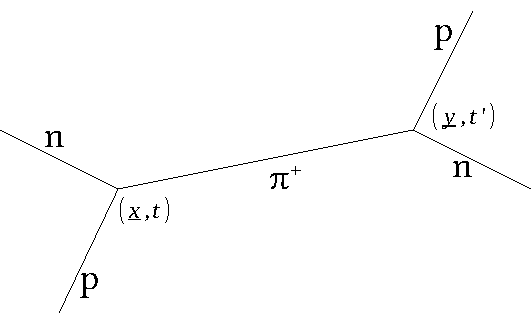
\includegraphics{Images/process.pdf}
\caption{Direct process of a proton-neutron scattering.}
\end{marginfigure}
These processes give the same initial and final states. From a quantum mechanical point of view, we have to sum over all the processes that give us same initial and final state. This operation is called the \textbf{vacuum expectation value of the time-ordered product of two operators}:
\begin{equation}
\labeq{tproduct}    
\bra{0}T[\Phi(x)\Phi^\dagger(y)]\ket{0}:=\theta(x^0-y^0)\bra{0}\Phi(x)\Phi^\dagger(y)\ket{0}+\theta(y^0-x^0)\bra{0}\Phi^\dagger(y)\Phi(x)\ket{0}\\
\end{equation}
The T-product is hence given by:
\begin{equation}
\labeq{tproductscalar}
T[\Phi(x)\Phi^\dagger(y)]=\theta(x^0-y^0)\Phi(x)\Phi^\dagger(y)+\theta(y^0-x^0)\Phi^\dagger(y)\Phi(x)\underset{\mathclap{\tikz \node {$\uparrow$} node [below=1ex] {\footnotesize this holds true for bosons };}}
=T[\Phi^\dagger(x)\Phi(y)]
\end{equation}
Now we can explicitly compute the object in \refeq{tproduct}:
\begin{align*}
\bra{0}T[\Phi(x)\Phi^\dagger(y)]\ket{0}=\int\frac{d^3pd^3p'}{(2\pi)^3\sqrt{4\omega\omega'}}&\left[\theta(x^0-y^0)e^{i(P_\mu y^\mu-P'_\mu x^\mu)}\bra{0}a_{p'}a^\dagger_p\ket{0}\right.\\
&+\left.\theta(y^0-x^0)e^{-i(P_\mu y^\mu+P'_\mu x^\mu)}\bra{0}b_pb^\dagger_{p'}\ket{0}\right]
\end{align*}
\begin{align*}
\bra{0}T[\Phi(x)\Phi^\dagger(y)]\ket{0}&=\int\frac{d^3p}{(2\pi)^32\omega}\left[\theta(x^0-y^0)e^{-iP_\mu(x-y)^\mu}+\theta(y^0-x^0)e^{iP_\mu(x-y)^\mu}\right]\\
&=-iD_F(x-y)
\end{align*}
We want to move to a more convenient and covariant way to express the Feynman propagator. To do this, we first rewrite the $\theta$ function as an integral:
\[
\theta(t)=\lim_{\eta\to0}\frac{i}{2\pi}\int_{-\infty}^{+\infty}d\omega\frac{e^{-i\omega t}}{\omega+i\eta}=\begin{cases}\text{upper plane: }t<0\Rightarrow\theta(t)=0\\ 
\text{lower plane: }t>0\Rightarrow\theta(t)=1
\end{cases}
\]
Taking into account this new way to write the $\theta$ function, we can express the Feynman propagator as:
\begin{align*}
-iD_F(x-y)&=i\int\frac{d^3p}{(2\pi)^4}\left\{\int\frac{d\omega}{2\omega_p}\left[\frac{e^{-i\omega(x^0-y^0)}e^{-iP_\mu(x-y)^\mu}}{\omega+i\eta}+\frac{e^{i\omega(x^0-y^0)}e^{iP_\mu(x-y)^\mu}}{\omega+i\eta}\right]\right\}\\
&=i\int\frac{d^4p}{(2\pi)^4}\frac{1}{2\omega_p}\left[\frac{e^{-ip^0(x^0-y^0)+\cancel{i\omega_p(x^0-y^0)}}e^{\cancel{-i\omega_p(x^0-y^0)}+ip(x-y)}}{P^0-\omega_p+i\eta}+\frac{e^{iP_\mu(x-y)^\mu}}{P^0-\omega_p+i\eta}\right]\\
&=i\int\frac{d^4p}{(2\pi)^42\omega_p}\left[\frac{e^{-iP_\mu(x-y)^\mu}}{P^0-\omega_p+i\eta}+\frac{e^{+iP_\mu(x-y)^\mu}}{P^0-\omega_p+i\eta}\right]\\
&=i\int\frac{d^4p}{(2\pi)^42\omega_p}e^{-iP_\mu(x-y)^\mu}\left[\frac{1}{P^0-\omega_p-i\eta}-\frac{1}{P^0+\omega_p-i\eta}\right]\\
&=i\int\frac{d^4p}{(2\pi)^4}\frac{e^{-iP_\mu(x-y)^\mu}}{2\omega_p(P^2-m^2+i\eta)}
\end{align*}
It is possible to show that this propagator satisfies \refeq{Greenfunc}:
\[
(\partial^2+m^2)D_F(x-y)=-\int\frac{d^4p}{(2\pi)^4}\cancelto{-1}{\frac{(-P^2+m^2)}{P^2-m^2}}e^{-iP(x-y)}=\delta^4(x-y)
\]
If we now compute the action of $(\partial^2+m^2)$ on the vacuum expectation value of the time-ordered product of the fields, what we get is:
\[
(\partial^2+m^2)_x\bra{0}T[\Phi(x)\Phi^\dagger(y)]\ket{0}=\partial_0^2\bra{0}T[\dots]\ket{0}+\bra{0}T[(-\nabla^2_x+m^2)\Phi(x)\Phi^\dagger(y)]\ket{0}
\]
From \refeq{tproduct}, remembering that the derivative acting on a $\theta$ function gives a $\delta$ function, we can rewrite the temporal term $\partial_0^2\bra{0}T[\dots]\ket{0}$ as:
\begin{align*}
\partial_0&\left\{\bra{0}\delta(x^0-y^0)\Phi(x)\Phi^\dagger(y)\ket{0}+\bra{0}\delta(y^0-x^0)\Phi^\dagger(y)\Phi(x)\ket{0}\right.\\
&\left.+\bra{0}\theta(x^0-y^0)\Dot{\Phi}(x)\Phi^\dagger(y)\ket{0}+\bra{0}\theta(y^0-x^0)\Phi^\dagger(y)\Dot{\Phi}(x)\ket{0}\right\}
\end{align*}
Putting this in a more convenient form gives us:
\[
\partial_0\left\{\bra{0}\delta(x^0-y^0)[\Phi(x),\Phi^\dagger(y)\ket{0}+\bra{0}\theta(x^0-y^0)[\Dot{\Phi}(x),\Phi^\dagger(y)\ket{0}\right\}
\]
Including now the spatial term leaves us with:
\begin{align*}
&\partial_0\left\{\bra{0}\delta(x^0-y^0)[\Phi(x),\Phi^\dagger(y)]\ket{0}\right\}+\bra{0}\delta(x^0-y^0)[\Dot{\Phi}(x),\Phi^\dagger(y)]\ket{0}\\
&+\bra{0}T(\partial_0^2[\Phi(x)\Phi^\dagger(y)])\ket{0}+\bra{0}T[(-\nabla^2_x+m^2)\Phi(x)\Phi^\dagger(y)]\ket{0}\marginnote{$\partial_0[\delta(x^0-y^0)F(x)]=\\-\Dot{F}(x)|_{x^0=y^0}+\delta(x^0-y^0)F(x)$.}\\
&=\cancel{-\bra{0}[\Dot{\Phi}(x),\Phi^\dagger(y)]_{x^0=y^0}\ket{0}}+\bra{0}\delta(x^0-y^0)[\Dot{\Phi}(x),\Phi^\dagger(y)]\ket{0}\\
&+\cancel{\bra{0}[\Dot{\Phi}(x),\Phi^\dagger(y)]_{x^0=y^0}\ket{0}}+\underline{\bra{0}T(\partial_0^2[\Phi(x)\Phi^\dagger(y)])\ket{0}}\\
&+\underline{\bra{0}T[(-\nabla^2_x+m^2)\Phi(x)\Phi^\dagger(y)]\ket{0}}\\
&=\bra{0}\delta(x^0-y^0)[\Dot{\Phi}(x),\Phi^\dagger(y)]\ket{0}+\underline{\bra{0}T[(\partial^2+m^2)\Phi(x)\Phi^\dagger(y)]\ket{0}}\marginnote{$[\Dot{\Phi}(\underline{x},t),\Phi^\dagger(\underline{y},t)]=-i\delta^3(\underline{x}-\underline{y})$}\\
&=-i\delta^4(x-y)+\bra{0}T[\cancelto{0}{(\partial^2+m^2)\Phi(x)}\Phi^\dagger(y)]\ket{0}=-i\delta^4(x-y)
\end{align*}
And we can conclude that:
\[
D_F(x-y)=i\bra{0}T[\Phi(x)\Phi^\dagger(y)]\ket{0}
\]
The result we obtained is the propagator of the \textbf{scalar field}, we want to find the propagators also for the \textbf{Dirac field} and for the \textbf{electromagnetic field}.
\subsection{Propagator for the Dirac field}
By analogy to the case of the scalar field, the Feynman propagator for the Dirac field turns out to be:
\[
S_F(x-y)_{\alpha\beta}=-i\bra{0}T[\Psi_\alpha(x)\bar{\Psi}_\beta(y)]\ket{0}
\]
In the scalar field case, the time-ordered product is the same if we exchange the two fields [\refeq{tproductscalar}] but in the fermion case this does not happen so we have to change the definition:
\[
T[\Psi_\alpha(x)\bar{\Psi}_\beta(y)]:=\theta(x^0-y^0)\Psi_\alpha(x)\bar{\Psi}_\beta(y){\color{red}-}\theta(y^0-x^0)\bar{\Psi}_\beta(y)\Psi_\alpha(x)
\]
It is \textbf{anti-symmetric} by definition, $T[\Psi_\alpha(x)\bar{\Psi}_\beta(y)]=-T[\bar{\Psi}_\beta(y)\Psi_\alpha(x)]$, because it has to satisfy anti-commutation relations. We want to prove that this is a Green's function for the Dirac equation [\refeq{Dirac}], therefore we apply the Dirac differential operator:
\begin{align*}
(i\slashed{\partial}_x-m)_{\alpha\beta}\bra{0}T[\Psi_\beta(x)\bar{\Psi}_\gamma(y)]\ket{0}&=\bra{0}i\gamma_{\alpha\beta}^0\delta(x^0-y^0)[\Psi_\beta(x),\bar{\Psi}_\gamma(y)]_+\ket{0}\\
&+\bra{0}T[i\gamma^0_{\alpha\beta}\partial_0\Psi_\beta(x)\bar{\Psi}_\gamma(y)]\ket{0}\\
&+\bra{0}T[(i\gamma^i_{\alpha\beta}\partial_i-m)\Psi_\beta(x)\bar{\Psi}_\gamma(y)]\ket{0}
\end{align*}
\begin{align*}
&=\bra{0}i\gamma_{\alpha\beta}^0\delta(x^0-y^0)[\Psi_\beta(x),\bar{\Psi}_\gamma(y)]_+\ket{0}+\cancel{\bra{0}(i\slashed{\partial}-m)\Psi_\beta(x)\bar{\Psi}_\gamma(y)\ket{0}}\\
&=\bra{0}i\gamma_{\alpha\beta}^0\delta(x^0-y^0)[\Psi_\beta(x),\bar{\Psi}_\gamma(y)]_+\ket{0}=\bra{0}i\gamma^0_{\alpha\beta}\delta_{\beta\delta}\delta^4(x-y)\gamma^0_{\delta\gamma}\ket{0}\marginnote{$[\Psi_\beta(x),\Psi^\dagger_\gamma(y)]_+=\delta_{\beta\gamma}\delta^3(x-y)$}\\
&=i\delta_{\alpha\gamma}\delta^4(x-y)
\end{align*}
It also possible to express the propagator in terms of integrals, by taking:
\[
S_F(x-y)=-(i\slashed{\partial}+m)D_F(x-y)
\]
Again, we apply the Dirac differential operator:
\begin{align*}
(i\slashed{\partial}-m)S_F(x-y)&=-(i\slashed{\partial}-m)(i\slashed{\partial}+m)D_F(x-y)\\
&=(\partial^2+m^2)D_F(x-y)=\delta^4(x-y)
\end{align*}
This means that the Feynman propagator for the Dirac field is:
\[
S_F(x-y)=-(i\slashed{\partial}+m)\int\frac{d^4p}{(2\pi)^4}\frac{e^{-iP_\mu(x-y)^\mu}}{P^2-m^2+i\eta}=\int\frac{d^4p}{(2\pi)^4}\frac{\slashed{P}+m}{P^2-m^2+i\eta}e^{-iP_\mu(x-y)^\mu}
\]
For the electromagnetic field, we have a massless scalar field. This translates into:
\[
\bra{0}T[A_\mu(x)A_\nu(y)]\ket{0}=i\eta_{\mu\nu}D_F(x-y) \quad D_F(x-y)=-\int\frac{d^4p}{(2\pi)^4}\frac{e^{-iP_\mu x^\mu}}{P^2+i\eta}
\]
\end{document} 